\RequirePackage{docswitch}
% \flag is set by the user, through the makefile:
%    make note
%    make apj
% etc.
\setjournal{\flag}

\documentclass[\docopts]{\docclass}

% You could also define the document class directly
%\documentclass[]{emulateapj}

% Custom commands from LSST DESC, see texmf/styles/lsstdesc_macros.sty
\usepackage{lsstdesc_macros}

\usepackage{graphicx}
\graphicspath{{./}{./figures/}}
\bibliographystyle{apj}

% Add your own macros here:



% ======================================================================

\begin{document}

\title{The Photometric LSST Astronomical Time-series Classification Challenge (PLAsTiCC): Selection of a performance metric balancing diverse science goals}

\maketitlepre

\begin{abstract}

  We describe and illustrate the process by which a global performance metric was chosen for Photometric LSST Astronomical Time-series Classification Challenge (PLAsTiCC), a Kaggle competition aiming to identify promising transient and variable classifiers for LSST by involving the broader community outside astronomy.

\end{abstract}

% Keywords are ignored in the LSST DESC Note style:
\dockeys{}

\maketitlepost

% ----------------------------------------------------------------------
% 

\section{Introduction}
\label{sec:intro}

The metric of this note is for the first version of the Kaggle competition, though there are future plans for an early classification challenge and identification of class-specific metrics for different science goals.

\begin{itemize}
\item    The metric must return a single scalar value.
\item    The metric must be well-defined for non-binary classes.
\item    The metric must balance diverse science use cases in the presence of heavily nonuniform class prevalence.
\item    The metric must respect the information content of probabilistic classifications.
\item    The metric must be able to evaluate deterministic classifications.
\item    The metric must be interpretable, meaning it gives a more optimal value for "good" mock classifiers and a less optimal value for mock classifiers plagued by anticipated systematic errors; in other words, it must pass basic tests of intuition.
\item    The metric must be reliable, giving consistent results for different instantiations of the same test case.
\end{itemize}

The Probabilistic Classification Metric (ProClaM) code used in this exploration of performance metrics is publicly available on GitHub.\footnote{\url{https://github.com/aimalz/proclam}}

\section{Data}
\label{sec:data}

We confirm the behavior of the metrics on mock data with well-understood systematics as well as real data from past classification challenges.

\subsection{Mock classifier systematics}
\label{sec:mockdata}

\begin{itemize}
\item    guessing: random classifications across all classes
\item    uncertain: uniform probabilities across all classes
\item    perfect: perfectly accurate on all classes
\item    almost: a slight perturbation of the perfect classifier
\item    noisy: a large perturbation of the perfect classifier
\item    tunnel vision: classifies one class well and others randomly
\item    cruise control: classifies all objects as a single class
\item    subsumed: consistently misclassifies one class as one other class
\end{itemize}

\subsubsection{}
\label{sec:guessing}

\subsubsection{}
\label{sec:uncertain}

\subsubsection{}
\label{sec:perfect}

\subsubsection{}
\label{sec:almost}

\subsubsection{}
\label{sec:noisy}

\subsubsection{}
\label{sec:tunnel}

\subsubsection{}
\label{sec:cruise}

\subsubsection{}
\label{sec:subsume}

\subsection{Representative classifications}
\label{sec:realdata}

\subsubsection{SNPhotCC}
\label{sec:snphotcc}

\subsubsection{Unknown}
\label{sec:mystery}

\section{Methods}
\label{sec:methods}

\subsection{Probabilistic metrics}
\label{sec:metrics}

We considered two metrics of classification probabilities, each of which is interpretable and avoids reducing probabilities to point estimates

The Brier score is defined as
\begin{eqnarray}
B &=& \sum_{m=1}^{M}\frac{w_{m}}{N_{m}}\sum_{n=1}^{N_{m}}\left((1-p_{n}(m | m))^{2}+\sum_{m'\neq m}^{M}(p_{n}(m' | m))^{2}\right)
\end{eqnarray}

The log-loss is defined as
\begin{eqnarray}
L &=& -\sum_{m=1}^{M}\frac{w_{m}}{N_{m}}\sum_{n=1}^{N_{m}}\ln[p_{n}(m | m)]
\end{eqnarray}

We calculate the metric within each class $m$ by taking an average of its value $-\ln[p_{n}(m | m)]$ for each true member $n$ of the class.  Then we weight the metrics for each class by an arbitrary weight $w_{m}$ and take a weighted average of the per-class metrics to produce a global scalar metric.

\subsection{Weights}
\label{sec:weights}

We may take weighted averages of the per-class metrics, and these weights may be considered in terms of the systematics we discussed, by upweighting or downweighting the "chosen" class most affected by the systematics.

\section{Results}
\label{sec:results}

\subsection{Mock classifier systematics}
\label{sec:mockresults}

\subsection{Representative classifications}
\label{sec:realresults}

\begin{figure*}
	\begin{center}
		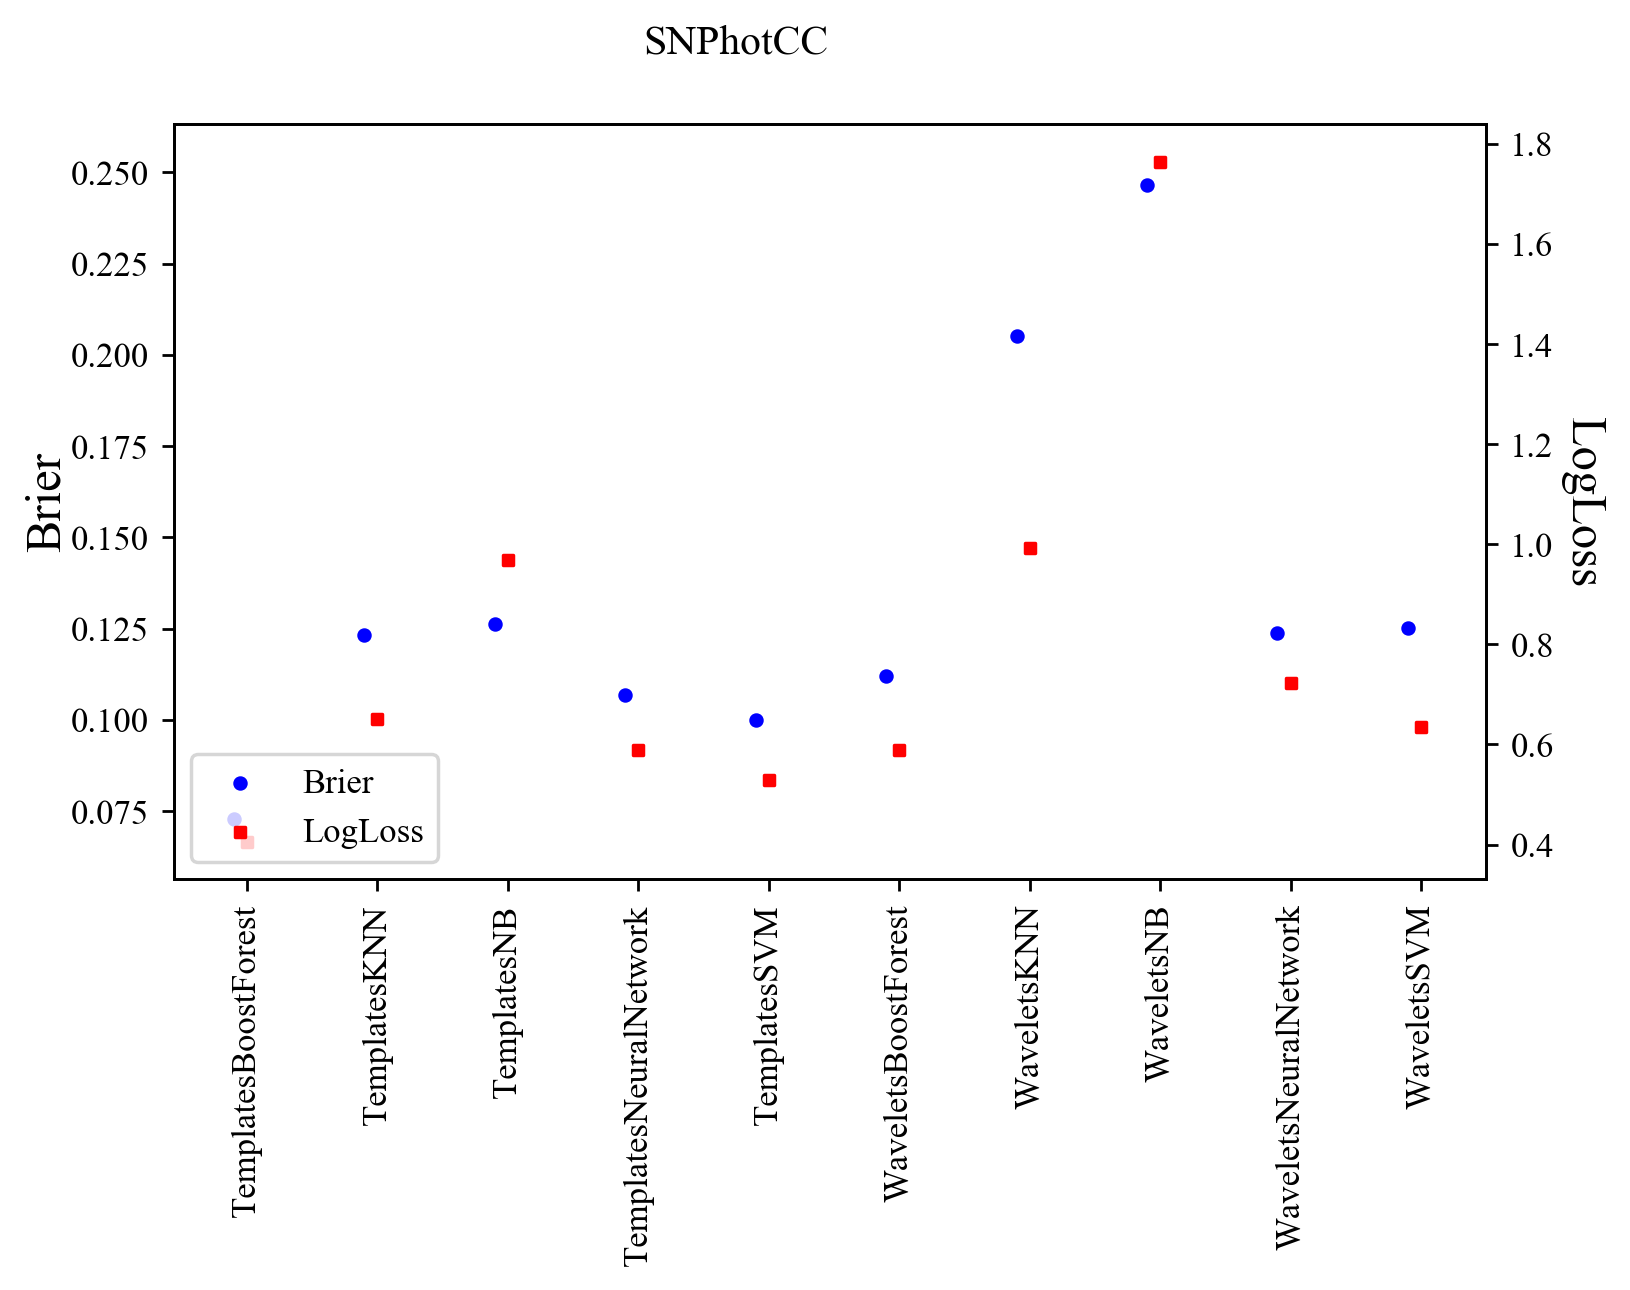
\includegraphics[width=\textwidth]{SNPhotCC.png}\\
		\caption{}
		\label{fig:snphotcc_metric_compare}
	\end{center}
\end{figure*}

\begin{figure*}
	\begin{center}
		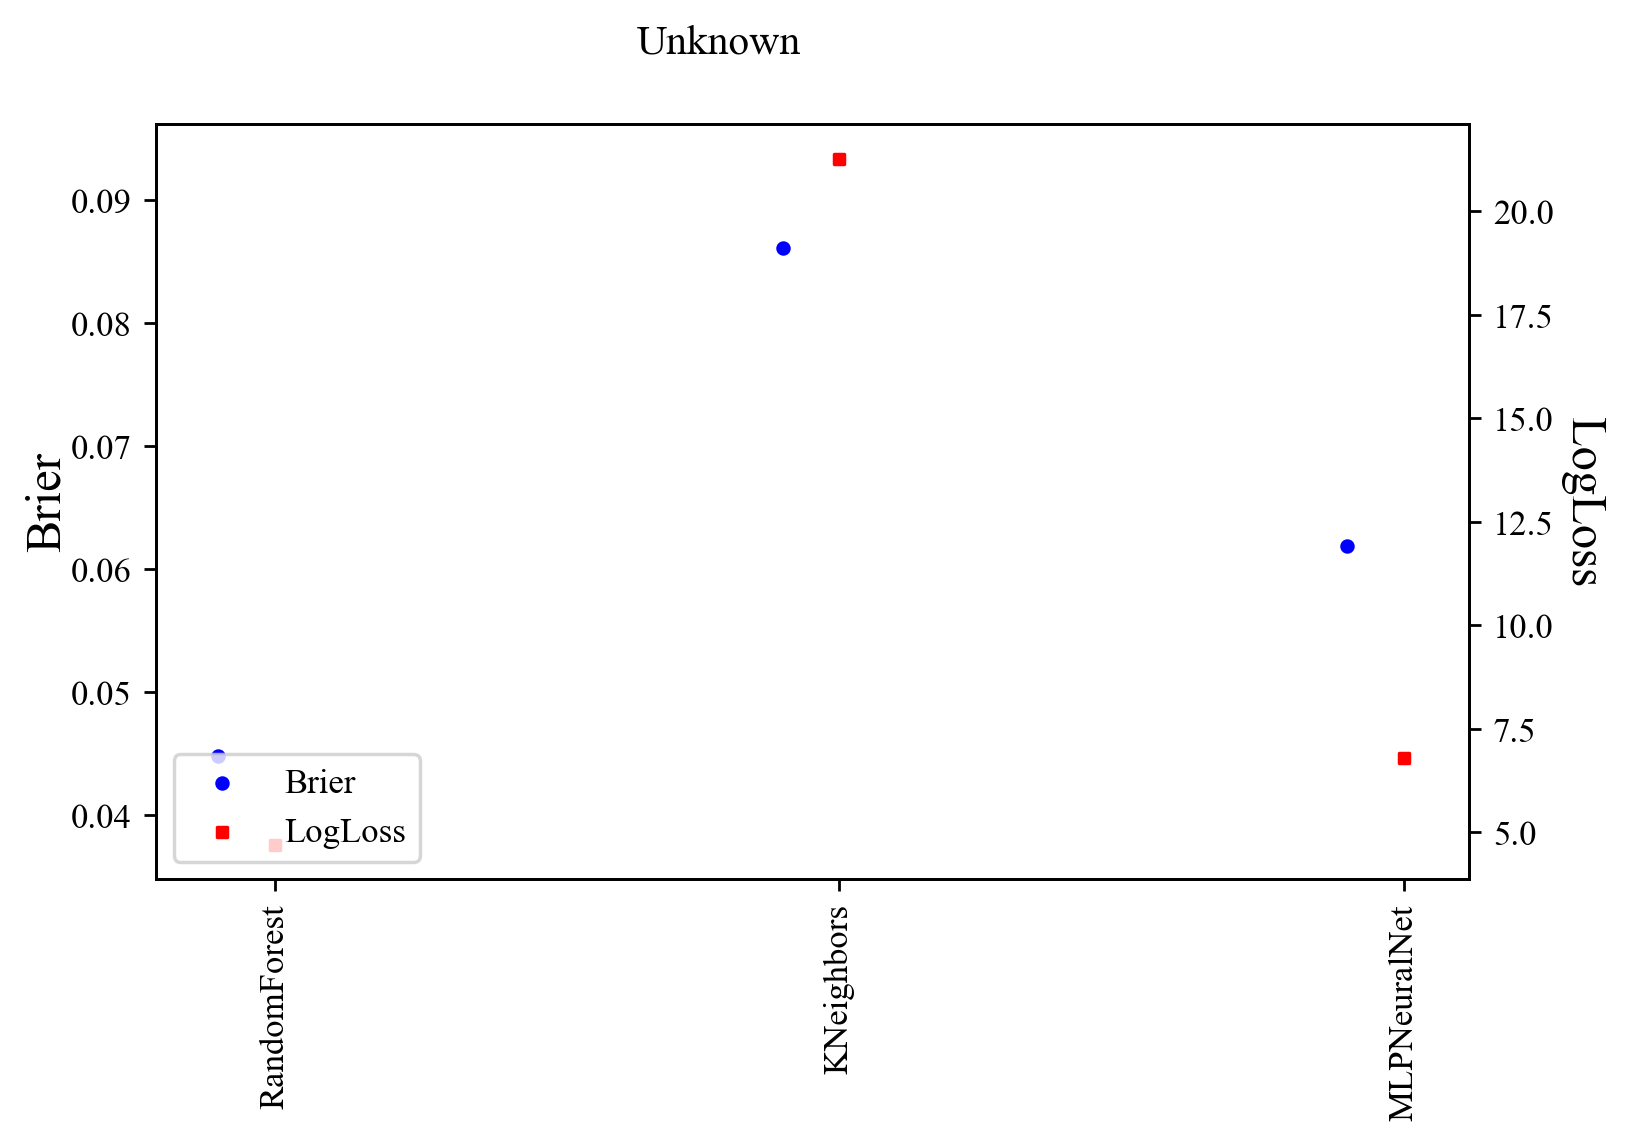
\includegraphics[width=\textwidth]{Unknown.png}\\
		\caption{}
		\label{fig:unknown_metric_compare}
	\end{center}
\end{figure*}

\section{Discussion}
\label{sec:discussion}



% ----------------------------------------------------------------------

\section{Conclusion}
\label{sec:conclusion}

We conclude that the Brier and log-loss metrics convey different information but are more or less consistent with our intuition for what makes a good classifier. The Brier metric includes a penalty term not present in the log-loss but somehow is always consistent with the log-loss, meaning the penalty term doesn't really make a difference. The log-loss has a larger dynamic range, which seems good but probably isn't that big a deal either.

% ----------------------------------------------------------------------

\subsection*{Acknowledgments}

%%% Here is where you should add your specific acknowledgments, remembering that some standard thanks will be added via the \code{desc-tex/ack/*.tex} and \code{contributions.tex} files.

%This paper has undergone internal review in the LSST Dark Energy Science Collaboration. % REQUIRED if true

Author contributions are listed below. \\
A.I.~Malz: conceptualization, data curation, formal analysis, investigation, methodology, project administration, software, supervision, validation, visualization, writing - original draft \\
R.~Hlozek: data curation, formal analysis, funding acquisition, investigation, project administration, software, supervision, validation, visualization, writing - original draft \\
T.~Alam: investigation, software, validation \\
A.~Bahmanyar: formal analysis, investigation, methodology, software, writing - original draft \\
R.~Biswas: conceptualization, methodology, software \\
E.E.O.~Ishida: conceptualization, project administration, supervision \\
G.~Narayan: data curation, formal analysis \\
D.~Jones: software \\
A.~Mahabal: data curation, software \\
R.~Martinez-Galarza: data curation, software, visualization \\
C.~Setzer: software \\
 % Standard papers only: author contribution statements. For examples, see http://blogs.nature.com/nautilus/2007/11/post_12.html

Alex Malz: conceptualization, data curation, formal analysis, investigation, methodology, project administration, software, supervision, validation, visualization, writing - original draft

Renee Hlozek: data curation, formal analysis, funding acquisition, investigation, project administration, software, supervision, validation, visualization, writing - original draft

Tarek Alam: investigation, software, validation

Anita Bahmanyar: formal analysis, investigation, methodology, software, writing - original draft

Rahul Biswas: conceptualization, methodology, software

Emille Ishida: conceptualization, project administration, supervision

David Jones: software

Ashish Mahabal: data curation, software

Rafael Martinez-Galarza: data curation, software, visualization

Gautham Narayan: data curation, formal analysis

% This work used TBD kindly provided by Not-A-DESC Member and benefitted from comments by Another Non-DESC person.

% Standard papers only: A.B.C. acknowledges support from grant 1234 from ...

The DESC acknowledges ongoing support from the Institut National de Physique Nucl\'eaire et de Physique des Particules in France; the Science \& Technology Facilities Council in the United Kingdom; and the Department of Energy, the National Science Foundation, and the LSST Corporation in the United States.  DESC uses resources of the IN2P3 Computing Center (CC-IN2P3--Lyon/Villeurbanne - France) funded by the Centre National de la Recherche Scientifique; the National Energy Research Scientific Computing Center, a DOE Office of Science User Facility supported by the Office of Science of the U.S.\ Department of Energy under Contract No.\ DE-AC02-05CH11231; STFC DiRAC HPC Facilities, funded by UK BIS National E-infrastructure capital grants; and the UK particle physics grid, supported by the GridPP Collaboration.  This work was performed in part under DOE Contract DE-AC02-76SF00515.
 % also available: key standard_short

% This work used some telescope which is operated/funded by some agency or consortium or foundation ...

The DESC acknowledges ongoing support from the Institut National de Physique Nucleaire et de Physique des Particules in France; the Science & Technology Facilities Council in the United Kingdom; and the Department of Energy, the National Science Foundation, and the LSST Corporation in the United States.

DESC uses resources of the IN2P3 Computing Center (CC-IN2P3--Lyon/Villeurbanne - France) funded by the Centre National de la Recherche Scientifique; the National Energy Research Scientific Computing Center, a DOE Office of Science User Facility supported by the Office of Science of the U.S. Department of Energy under Contract No. DE-AC02-05CH11231; STFC DiRAC HPC Facilities, funded by UK BIS National E-infrastructure capital grants; and the UK particle physics grid, supported by the GridPP Collaboration.

This work was performed in part under DOE Contract DE-AC02-76SF00515.

% We acknowledge the use of An-External-Tool-like-NED-or-ADS.

%{\it Facilities:} \facility{LSST}

% Include both collaboration papers and external citations:
\bibliography{main,lsstdesc}

\end{document}

% ======================================================================
